\documentclass{standalone}
\usepackage{tikz}
\usepackage{verbatim}
\usetikzlibrary{intersections}
\begin{document}
\pagestyle{empty}
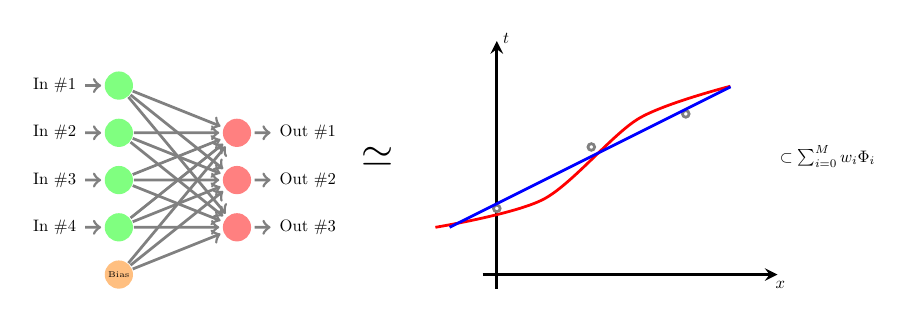
\begin{tikzpicture}[scale=0.6, transform shape, shorten >=1pt,->,draw=black!50, node distance=2.5cm, line width=1pt]
    \tikzstyle{every pin edge}=[<-,shorten <=1pt]
    \tikzstyle{neuron}=[circle,fill=black!25,minimum size=17pt,inner sep=0pt]
    \tikzstyle{input neuron}=[neuron, fill=green!50];
    \tikzstyle{output neuron}=[neuron, fill=red!50];
    \tikzstyle{bias neuron}=[neuron, fill=orange!50];
    \tikzstyle{annot} = [text width=4em, text centered]
    % Draw the input layer nodes
    \foreach \name / \y in {1,...,4}
        \node[input neuron, pin=left:In \#\y] (I-\name) at (0,-\y+5) {};
    \node[bias neuron] (B-1) at (0,0) {\tiny{Bias}};
    % Draw the output layer node
    \foreach \name / \y in {1,...,3}
        \path[yshift=-1cm]
            node[output neuron,pin={[pin edge={->}]right:Out \#\y}] (O-\name) at (2.5cm,-\y+5) {};
    % Connect every node in the input layer with every node in the hidden layer.
    \foreach \source in {1,...,4}
        \foreach \dest in {1,...,3}
            \path (I-\source) edge (O-\dest);
    \foreach \dest in {1,...,3}
        \path (B-1) edge (O-\dest);

  \coordinate (O) at (0,0);
  \draw[-stealth, black] (7.7,0) -- (14,0) coordinate[label = {below:$x$}] (xmax);
  \draw[-stealth, black] (8,-.3) -- (8,5) coordinate[label = {right:$t$}] (ymax);
  \path[name path=x] (7.3,0.5) -- (13.7,4.7);
  \path[name path=y] plot[smooth] coordinates {(6.7,2) (9,1.5) (11,2.8) (13,5)};
  \draw[-,red] plot[smooth] coordinates {(6.7,1) (9,1.6) (11,3.3) (13,4)};
  \draw[-] (8,1.4) node[draw,fill = white,circle,inner sep = 0pt,minimum size = 4pt] {}  (10,2.7) node[draw,fill = white,circle,inner sep = 0pt,minimum size = 4pt] {} (12,3.4) node[draw,fill = white,circle,inner sep = 0pt,minimum size = 4pt] {};
  \draw[-,blue] (7,1) -- (13,4);
  \node[right] at (5,2.5) {\Huge{$\simeq$}};

  \node at (15,2.5) {$\subset \sum_{i=0}^{M} w_i \Phi_i$};

\end{tikzpicture}
\end{document}